\chapter{Analysis of existing corporation}

As an example of an existing service implementation let's take an anonymous company. For the purpose of this thesis it will be named Invest s.r.o.. The company is operating on the market more than ten years and during this period was reorganised to service-oriented architecture. Invest s.r.o. has many clients in its portfolio. Many of them are consuming services provided by this company.

\section{Architecture overview}
Architecture of Invest s.r.o. can be divided into multiple layers. In sake of providing services to the third party the application is composed by Data layer, Application layer, Integration layer as is shown on Figure \ref{fig:invest-architecture}.

\begin{figure}[htp] \centering{
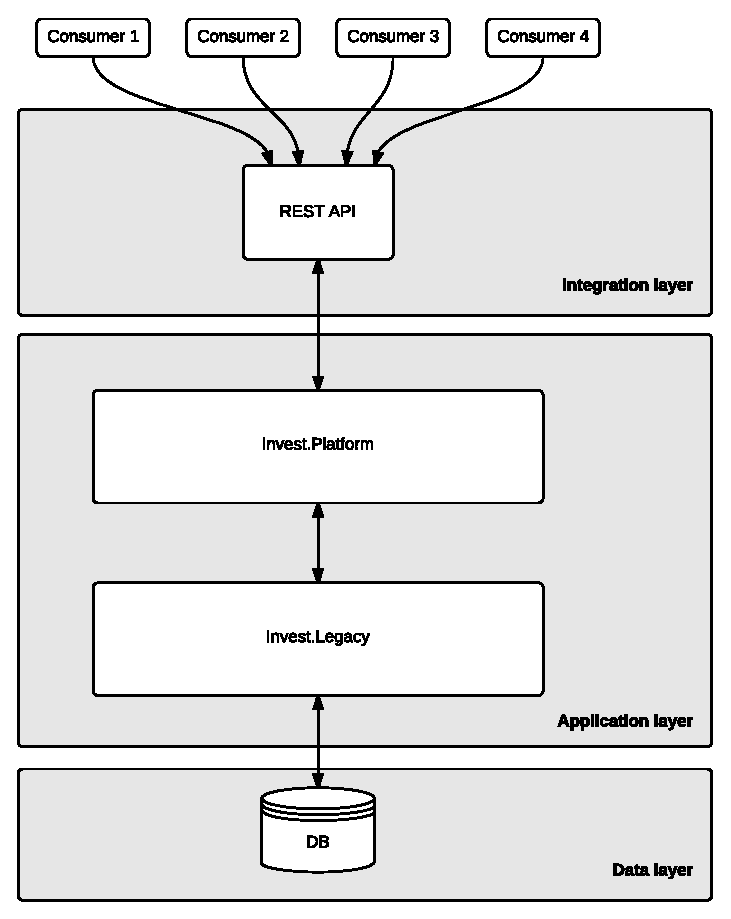
\includegraphics[width=8cm]{img/invest-architecture.pdf}}
\caption{Invest s.r.o. architecture}
\label{fig:invest-architecture}
\end{figure} 

The highest layer of application is Integration layer containing service API. It provides access points to underlying logic. Services consumers integrate it to their applicaton. The Application layer holds the whole business logic. Every logical functionality is performed in this layer. Data are stored within Data layer.

\section{Integration layer}
Services of Invest s.r.o. are REST-based. The HTTP methods are used for communication between the company and its clients. A service is accessed by URL template and HTTP verbs such as GET, POST, PUT and DELETE. For example, to retrieve a bank account with concrete id the service call looks as follows: 

\begin{lstlisting}
    GET    /api/bankaccounts/{bankAccountId}
\end{lstlisting}

In call the \emph{\{bankAccountId\}} part of URL is replaced by bank account identifier which the client wants to obtain in response.

HTTP messages can be sent in XML or JSON format. Services are able to process both of them. Headers like Content-type and Accept can be filled by one of them:
 
\begin{lstlisting}
    Content-type: application/json
    Accept: application/json
\end{lstlisting}

Invest s.r.o service API contains many sarvices. Every of them is available for clients. Client can take set of services to compose a business processes. As an expamle, client has a login process through which an user passes to access his user account. User has to provide the user name, user password and memorable word. After filling them correctly the user can operate with his account. Client has to sent these requests:

\begin{lstlisting}
    POST /api/session
    POST /api/memorablewords
\end{lstlisting}
  
This process is composed by two services. The first of them authenticates the credentials and starts the session. The other one make another identity check. It posts the user's answer to asked memorable word characters. When both requests pass, obtaining the response code 200 OK, the user is logged in to his account.

\section{Versioning of services}
The versioning strategy of Invest s.r.o is based on avoiding the breaking changes. It is trying to not influence the consumers of services. This is ensured by only backward compatible changes within the service interface. After a certain amount of changes it is created the new version of API. This version is then present in URL. 

\subsection{API version in URL}
The company is versioning whole srvice API. The approach to versioning is the one which is used to version softvares in general. When a new version is created and deployed to production environment the old version is no longer accessible. The version paremeter in URL is informative. It can suggest to clients that they have to call requests according to \gls{documentation} of this API version.

\subsection{Service interface changes}
When it is needed to change a service interface the company tries to not affect any of its clients. For example after a change in implementation of service one of the attributes of representation doesn't hold enough information anymore. There is a need to encapsulate this attribute into another one. Let's have bank account. The original representation in request is:

\begin{lstlisting}
  <?xml version="1.0"?>
  <BankAccount>
    <BankAccountId>1</BankAccountId>
    <BankAccountNumber>12345678</BankAccountNumber>
    <BankName>InvestBank</BankName>
    <BankAccountName>MyBankAccount</BankAccountName>
  </BankAccount>
\end{lstlisting}

After a change of the requirements there is a need to have \emph{BankAddress} attribute in representation. \emph{BankAddress} and \emph{BankName} will be encapsulated into the node \emph{bankDetails}. The new request than should look like:

\begin{lstlisting}
  <?xml version="1.0"?>
  <BankAccount>
    <BankAccountId>1</BankAccountId>
    <BankAccountNumber>12345678</BankAccountNumber>
    <BankDetails>
      <BankName>InvestBank</BankName>
      <BankAddress>
        <Line1>Road 12</Line1>
        <Line2>London</Line2>
        <PostCode>AA0000A</PostCode>
      </BankAddress>
    </BankDetails>
    <BankAccountName>MyBankAccount</BankAccountName>
  </BankAccount>
\end{lstlisting}

If the change will be deployed it will harm the usability of application for each client who expect the old version. It is a breaking change which would force all clients to integrate this change or the provider to create a new version of a service. The Invest s.r.o. solve this by adding a new attribut with the encapsulation. At the same time the old attribute is left in the representation and is signed as obsolete.

\begin{lstlisting}
  <?xml version="1.0"?>
  <BankAccount>
    <BankAccountId>1</BankAccountId>
    <BankAccountNumber>12345678</BankAccountNumber>
    <BankName>InvestBank</BankName>
    <BankDetails>
      <BankName>InvestBank</BankName>
      <BankAddress>
        <Line1>Road 12</Line1>
        <Line2>London</Line2>
        <PostCode>AA0000A</PostCode>
      </BankAddress>
    </BankDetails>
    <BankAccountName>MyBankAccount</BankAccountName>
  </BankAccount>
\end{lstlisting}

Both attributes has to be optional because clients make calls just with one of them. In service implementation the code for both kind of calls has to be present. This way the API is becoming big and has many code to maintainance. 

At some point it occurs than there will be new version if API. All the duplications within a represenation and the code are removed. The version of API is increased and it is created a new service documentation.

This approach is offering enough time to clients to integrate the changes. 













